
\documentclass[11pt,a4paper]{article}
\usepackage[utf8]{inputenc}
\usepackage[T1]{fontenc}
\usepackage[spanish,es-nodecimaldot]{babel}
\usepackage[a4paper,left=1.7cm,right=1.7cm,top=20mm,bottom=20mm]{geometry}
\usepackage{amsmath,amssymb,amsfonts,mathtools,bm}
\usepackage{braket}
\usepackage{graphicx}
\usepackage{float}
\usepackage{booktabs}
\usepackage{enumitem}
\usepackage{xcolor}
\usepackage{lmodern,microtype}
\usepackage{fancyhdr}
\usepackage{titlesec}
\usepackage[colorlinks=true,linkcolor=black,urlcolor=black,citecolor=black]{hyperref}
\numberwithin{equation}{section}
\renewcommand{\boxed}[1]{#1}
\setlength{\parindent}{0pt}
\setlength{\parskip}{5pt}
\newcommand{\dd}{\,\mathrm d}
\newcommand{\ii}{\mathrm i}
\newcommand{\e}{\mathrm e}
\newcommand{\hb}{\hbar}
\newcommand{\R}{\mathbb R}
\newcommand{\C}{\mathbb C}
\newcommand{\id}{\mathbb I}

\pagestyle{fancy}
\setlength{\headheight}{14pt}
\fancyhf{}
\fancyhead[L]{\textit{Tarea 18}}
\fancyhead[R]{Mecánica Cuántica I}
\begin{document}
\begin{titlepage}
\centering
\vspace*{1.8cm}

\includegraphics[width=.22\textwidth]{UdeC_escudo.png}
\vspace{1.1cm}
{\Huge\bfseries Tarea 18\par}
\vspace{.4cm}
{\Huge\bfseries Mecánica Cuántica I\par}
\vspace{1.5cm}
{\Large José Ignacio Rosas Sepúlveda\par}
\vspace{.8cm}
{\Large Solución\par}
\vfill
\thispagestyle{empty}
\end{titlepage}
\tableofcontents
\newpage
\section*{Enunciado}
\addcontentsline{toc}{section}{Enunciado}
\begin{enumerate}[label=\arabic*.-]
\item Demuestre que los dos estados propios (16) del operador reducido son ortogonales.
\item Considere dos qubits en el estado puro
\begin{equation}
\ket\psi=N\left(\ket-_1\ket\downarrow_2+i\alpha\ket\downarrow_1\ket-_2\right),
\qquad \alpha\in\mathbb R,
\end{equation}
donde $N>0$.
\begin{enumerate}[label=\alph*)]
\item Encuentre $N$.
\item Calcule la concurrencia $C(\ket\psi)$.
\item Calcule $\rho_1$.
\item Calcule los valores propios de $\rho_1$.
\item Calcule la pureza $\operatorname{Tr}(\rho_1^2)$.
\item Calcule la entropía de von Neumann $S(\rho_1)$.
\item Grafique concurrencia, pureza y entropía como funciones de $\alpha$ y comente.
\end{enumerate}
\item Para el estado de Werner
\begin{equation}
\rho_W=\frac{1-\gamma}{4}I+\gamma\ket{\psi_+}\bra{\psi_+},
\qquad 0\le\gamma\le1,
\end{equation}
con $\ket{\psi_+}=(\ket{\downarrow\uparrow}+\ket{\uparrow\downarrow})/\sqrt2$, calcule la concurrencia y grafique $C(\gamma)$ y el entrelazamiento de formación $E(\gamma)$.
\end{enumerate}


\section{Problema 1}
El operador estado reducido $\rho_1$ es hermítico. Sean $\ket{\lambda_+}$ y $\ket{\lambda_-}$ estados propios asociados a valores distintos $\lambda_+\neq\lambda_-$. Entonces
\begin{align}
\braket{\lambda_-|\rho_1|\lambda_+}&=\lambda_+\braket{\lambda_-|\lambda_+},\\
\braket{\lambda_-|\rho_1|\lambda_+}&=\lambda_-\braket{\lambda_-|\lambda_+},
\end{align}
porque $\rho_1=\rho_1^\dagger$. Restando ambas ecuaciones,
\begin{equation}
(\lambda_+-\lambda_-)\braket{\lambda_-|\lambda_+}=0.
\end{equation}
Como los valores son distintos,
\begin{equation}
\boxed{\braket{\lambda_-|\lambda_+}=0.}
\end{equation}

\section{Problema 2}
El estado es
\begin{equation}
\ket\psi=N\left(\ket{-}_1\ket\downarrow_2+\ii\alpha\ket\downarrow_1\ket{-}_2\right),
\qquad \alpha\in\R.
\end{equation}
Expandiendo en la base $z$ se obtiene
\begin{equation}
\ket\psi=\frac{N}{\sqrt2}
\left(\ket{\uparrow\downarrow}+\ii\alpha\ket{\downarrow\uparrow}
-(1+\ii\alpha)\ket{\downarrow\downarrow}\right).
\end{equation}
La normalización da
\begin{equation}
\boxed{N=\frac1{\sqrt{1+\alpha^2}}.}
\end{equation}
La concurrencia de este estado puro es
\begin{equation}
\boxed{C(\psi)=\frac{|\alpha|}{1+\alpha^2}.}
\end{equation}

El operador reducido puede escribirse matricialmente en $\{\ket\uparrow,\ket\downarrow\}$ como
\begin{equation}
\rho_1=\frac{1}{2(1+\alpha^2)}
\begin{pmatrix}
1&-(1-\ii\alpha)\\
-(1+\ii\alpha)&1+2\alpha^2
\end{pmatrix}.
\end{equation}
Sus valores propios, como corresponde a cualquier estado puro de dos qubits, son
\begin{equation}
\boxed{\lambda_\pm=\frac12\left(1\pm\sqrt{1-C^2}\right).}
\end{equation}
La pureza es
\begin{equation}
\boxed{\operatorname{Tr}\rho_1^2=1-\frac{C^2}{2}.}
\end{equation}
La entropía de von Neumann, usando logaritmo base dos, es
\begin{equation}
\boxed{S(\rho_1)=-\lambda_+\log_2\lambda_+-\lambda_-\log_2\lambda_-.}
\end{equation}
\begin{figure}[H]\centering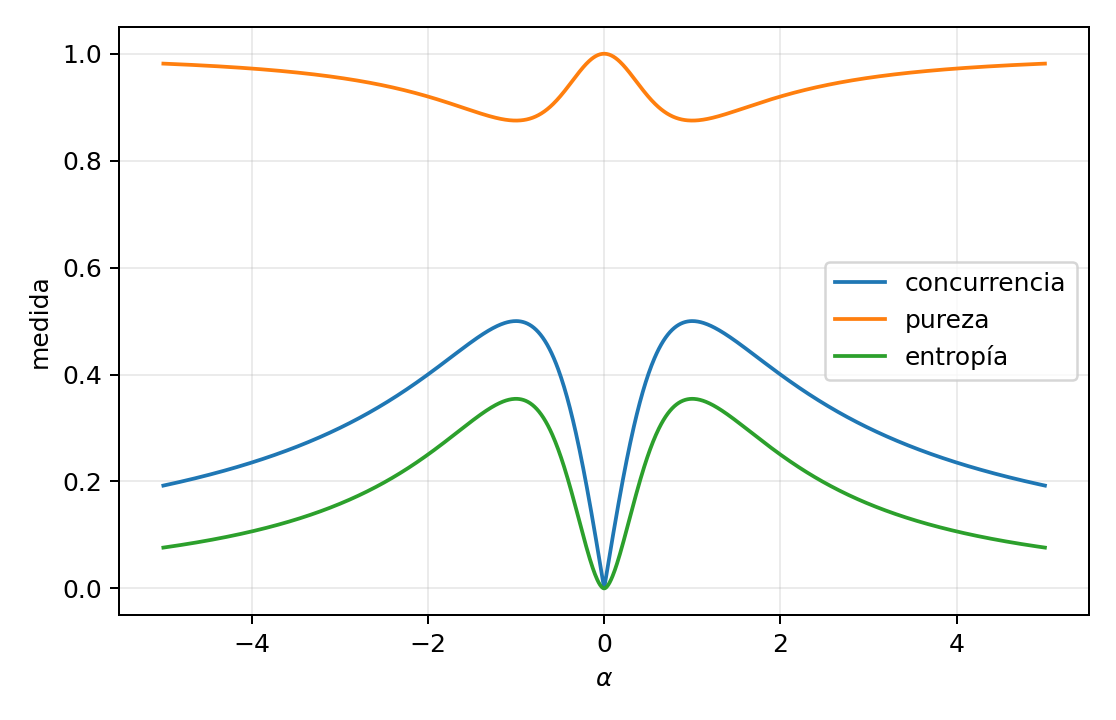
\includegraphics[width=.70\textwidth]{figures/entrelazamiento_alpha.png}\caption{Concurrencia, pureza y entropía del subsistema.}\end{figure}

\section{Problema 3}
Para
\begin{equation}
\rho_W=\frac{1-\gamma}{4}\id+\gamma\ket{\psi_+}\bra{\psi_+},
\qquad0\le\gamma\le1,
\end{equation}
la concurrencia conocida para esta familia se obtiene de la matriz ``spin-flipped'' y resulta
\begin{equation}
\boxed{C(\rho_W)=\max\left\{0,\frac{3\gamma-1}{2}\right\}.}
\end{equation}
El entrelazamiento de formación es
\begin{equation}
\boxed{E(\rho_W)=h_2\left(\frac{1+\sqrt{1-C^2}}{2}\right),}
\end{equation}
donde $h_2(x)=-x\log_2x-(1-x)\log_2(1-x)$.
\begin{figure}[H]\centering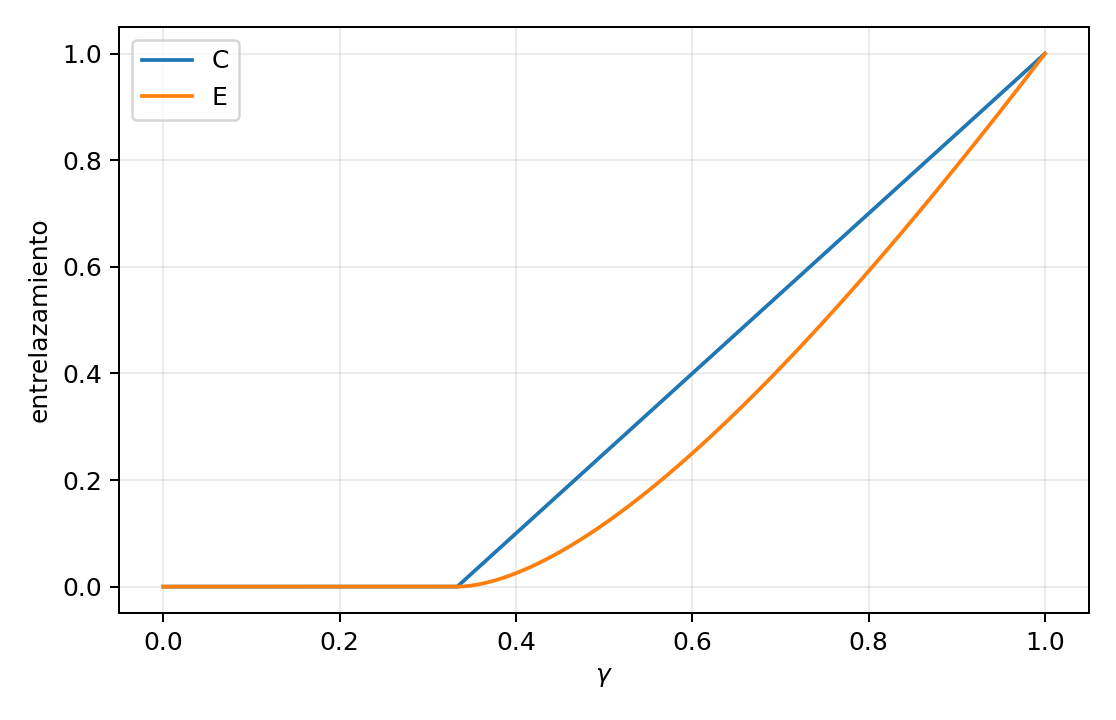
\includegraphics[width=.68\textwidth]{figures/werner.png}\caption{Concurrencia y entrelazamiento de formación del estado de Werner.}\end{figure}
El umbral $\gamma=1/3$ separa la región separable de la región entrelazada.


\end{document}
